\subsection{Nouveautés de la version 1.1 de 3D Tiles}

Avec la nouvelle version 1.1 de la spécification 3D Tiles, il a été introduit une nouvelle fonctionnalité appelée \textit{Implicit Tiling}. Elle permet de diviser implicitement un dataset en tuiles de mêmes tailles sans avoir à les définir explicitement.

Pour cela, l'implicit tiling divise la carte en tuiles de manière récursive. Tant que le \texttt{level} de division n'a pas atteint la valeur maximum \texttt{availableLevels}, on divise la tuile dans laquelle nous nous trouvons en tuiles de même taille.

Deux méthodes de division sont actuellement disponibles : \texttt{QUADTREE} et \texttt{OCTREE}. La première reste sur un concept de tuiles en deux dimensions, tandis que les octrees permettent de diviser les tuiles en rajoutant une notion de hauteur, donc en 3 dimensions. Dans mon cas, j'utilise une division en quadtree puisque tout les bâtiments que je dois traiter se trouvent sur un plan 2D.

\begin{figure}[H]
    \centering
    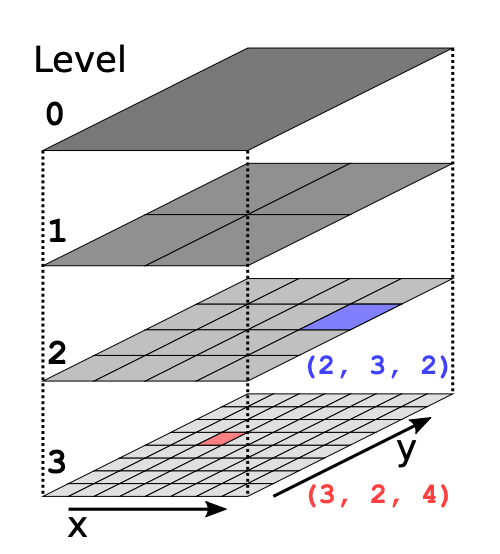
\includegraphics[width=0.4\textwidth]{assets/figures/implicit-tiling-small.png}
    \caption{Division en quadtree par implicit tiling \cite{3d-tiles-specification}}
    \label{fig:implicit-tiling}
\end{figure}

Le niveau 0 englobe l'entièreté du Tileset, dans notre cas la planète entière, puis, à chaque division, chaque tuile correspond non pas à une profondeur supplémentaire, mais à une portion de plus en plus petite du Tileset. Ainsi, une tuile de \texttt{level} 0 est la tuile de base, une tuile de \texttt{level} 1 est une tuile résultant de la division de la tuile de \texttt{level} 0, etc. Plus d'informations quand à l'indexation des tuiles sont disponibles dans la section \ref{sec:morton}.

Pour définir un implicit tiling, il faut en premier lieux créer un Tileset hôte qui définira entre autre son \texttt{bounding volume}. L'implicit tiling va ensuite définir les tuiles de ce Tileset hôte en fonction de son \texttt{subdivisionScheme}, de son \texttt{subtreeLevels} et de ses \texttt{availableLevels}, tout en prenant comme taille initiale le \texttt{bounding volume} du Tileset. Enfin, il est possible de définir les adresses auxquelles le client doit envoyer des requêtes pour obtenir les tuiles ainsi que les \textit{Subtrees}. Ces derniers seront discutés dans leur chapitre dédié \autoref{sec:subtrees-intro}. Selon la spécification, le client Cesium s'attend à recevoir des fichiers glb (glTF binary) pour les tuiles.

\newpage
Ci-dessous un exemple de fichier JSON définissant un Tileset avec un implicit tiling :

\begin{verbatim}
{
    "asset" : {
        "version" : "1.1"
    },
    "geometricError": 1200000,
    "root" : {
        "boundingVolume": {
            "region": [-3.14, -1.57, 3.14, 1.57, 0, 60]
        },
        "refine": "REPLACE",
        "geometricError": 1200000,
        "content": {
        "uri" : "/content/content_glb_{level}__{x}_{y}.glb"
        },
        "implicitTiling" : {
            "subdivisionScheme" : "QUADTREE",
            "subtreeLevels" : 4,
            "availableLevels" : 19,
            "subtrees" : {
                "uri" : "/subtrees/{level}.{x}.{y}.subtree"
            }
        }
    }
}
\end{verbatim}

En plus de l'implicit tiling, la version 1.1 de 3D Tiles apporte le support des fichiers glTF ainsi que deux nouvelles extensions : \href{https://github.com/CesiumGS/glTF/tree/3d-tiles-next/extensions/2.0/Vendor/EXT_mesh_features}{EXT\_mes\_features}\footnote{https://github.com/CesiumGS/glTF/tree/3d-tiles-next/extensions/2.0/Vendor/EXT\_mesh\_features} et \href{https://github.com/CesiumGS/glTF/tree/3d-tiles-next/extensions/2.0/Vendor/EXT_structural_metadata}{EXT\_structural\_metadata}\footnote{https://github.com/CesiumGS/glTF/tree/3d-tiles-next/extensions/2.0/Vendor/EXT\_structural\_metadata}. Cela introduit beaucoup de nouvelles possibilités par rapport à l'ancien système, notamment à des \textit{metadata} très précises par objet glTF.

Bien que la génération de fichiers glTF sera discuté dans la section \ref{sec:gltf}, je ne parlerai pas des extensions dans ce rapport puisqu'elles n'ont pas été utilisées dans mon projet.

\newpage
\subsection{Avantages et inconvénients de l'implicit tiling}

Comme son nom l'indique, cette technique de division de tuiles est implicite, ce qui signifie que l'on ne peut pas définir nous même les caractéristiques des tuiles. Cela peut être un avantage pour des datasets très grands, comme une planète entière, où il serait difficile de définir explicitement les tuiles, mais cela peut poser problème lorsque le \texttt{bounding volume} d'une tuile contenant une petite maison de campagne sera le même que celui de la tuile qui contiendra l'Empire State Building. Un autre point bénéfique à être définit explicitement par tuile est les niveaux de détails. En reprenant le même exemple, il serait intéressant de pouvoir définir que la tuile contenant l'Empire State Building doit contenir plusieurs niveaux de détails tandis que la tuile contenant la maison de campagne n'en a besoin que d'un seul. En utilisant l'implicit tiling, une tuile ne contiendra forcément qu'un seul niveau de détail définit implicitement. Une tuile définit explicitement peut quant à elle contenir plusieurs niveaux de détails sous la forme d'une chaîne de tuiles (liées entre elles par leur champ \texttt{children}). Plus d'informations sur les niveaux de détails et les \texttt{geometric error} sont disponibles dans la section \ref{sec:lod}.

% TODO: schema vu de côté ?

Du bon côté, l'implicit tiling permet d'effectuer tous ces calculs de \texttt{bounding volume} et de \textt{geometric error} de manière extrêmement rapide en ne se basant que sur la tuile parente plutôt que de devoir analyser la database et calculer ces valeurs en fonction des objets qu'elle contient.

Un entre-deux serait d'utiliser l'implicit tiling pour les tuiles de plus haut niveau, puis de définir explicitement les tuiles de plus bas niveau ou alors des tuiles spécifiques qui nous intéresserait principalement. Cela permettrait de profiter des avantages des deux méthodes. Actuellement, il est possible de fournir des nouveaux Tilesets à la place de fichier glb à un client qui effectuerait des requêtes sur la base d'un implicit tiling. Cette fonctionnalité n'est néanmoins absolument pas décrite dans la spécification 3D Tiles. Il ne faut donc actuellement pas la considérer comme une fonctionnalité stable ou supportée par Cesium.

J'ai cependant fait quelques tests en l'utilisant, initialement par accident. Je n'ai malheureusement pas réussi à obtenir un résultat satisfaisant. Les \texttt{bounding volumes} des tuiles générés par mes soins n'étaient pas du tout pris en compte par le client Cesium, ce qui posait de gros problèmes lors du calcul du niveau de détail à afficher. De plus, lorsque la caméra avait certains angles de vue, les tuiles étaient déchargées et enlevées de l'affichage. Je suspecte que cela soit partiellement dû aux mauvais \texttt{bounding volumes} attribués aux tuiles. Une différence entre une vue vers le Nord et une vue vers le Sud affectait aussi la visibilité des tuiles, ce qui me laisse penser que d'autres paramètres doivent aussi entrer en jeu.